%%%%%%%%%%%%%%%%%%%%%%%%%%%%%%%%%%%%%%%%%%%%%%%%%%%%%%%%%%%%%%%%%%%%%%%%%%%%%%
%%%%%%%%%%%%%%%%%%%%%%%%%%%%%%%%%%%%%%%%%%%%%%%%%%%%%%%%%%%%%%%%%%%%%%%%%%%%%%
%%
%% Ukázkový příklad dokumentace úkolu do předmětů IZP a IUS, 2010
%%
%% Upravená původní dokumentace od Davida Martinka.
%%%%%%%%%%%%%%%%%%%%%%%%%%%%%%%%%%%%%%%%%%%%%%%%%%%%%%%%%%%%%%%%%%%%%%%%%%%%%%
%%%%%%%%%%%%%%%%%%%%%%%%%%%%%%%%%%%%%%%%%%%%%%%%%%%%%%%%%%%%%%%%%%%%%%%%%%%%%%
\documentclass[12pt,a4paper,titlepage,final]{article}

% cestina a fonty
\usepackage[czech]{babel}
\usepackage[utf8]{inputenc}
% balicky pro odkazy
\usepackage[bookmarksopen,colorlinks,plainpages=false,urlcolor=blue,unicode]{hyperref}
\usepackage{url}
% obrazky
\usepackage[dvipdf]{graphicx}
% velikost stranky
\usepackage[top=3.5cm, left=2.5cm, text={17cm, 24cm}, ignorefoot]{geometry}

\begin{document}

%%%%%%%%%%%%%%%%%%%%%%%%%%%%%%%%%%%%%%%%%%%%%%%%%%%%%%%%%%%%%%%%%%%%%%%%%%%%%%
% titulní strana

% !!!!!!!!!!!!!!!!!!!!!!!!!!!!!!!!!!!!!!!!!!!!!!!!!
% změň následující údaje za své
\def\author{Roman Blanco}
\def\email{xblanc01X@stud.fit.vutbr.cz}
\def\projname{Iterační výpočty}
% !!!!!!!!!!!!!!!!!!!!!!!!!!!!!!!!!!!!!!!!!!!!!!!!!

\begin{titlepage}

	% \vspace*{1cm}
	\begin{figure}[!h]
	  \centering
	  
\includegraphics[height=5cm]{img/logo.eps}
	\end{figure}

	\vfill

	\begin{center}
		\begin{Large}
			ITO - Teorie obvodů\\
		\end{Large}
		\bigskip
			\begin{Huge}
				\projname\\
			\end{Huge}
		\begin{large}
			Řešení zadaných obvodů
		\end{large}
	\end{center}

	\vfill

	\begin{center}
		\begin{Large}
			\today
		\end{Large}
	\end{center}

	\vfill

	\begin{flushleft}
		\begin{large}
			\begin{tabular}{ll}
			Autor: & \author, \url{\email} \\
			 & Fakulta Informačních Technologií \\
			 & Vysoké Učení Technické v~Brně \\
			\end{tabular}
		\end{large}
	\end{flushleft}
\end{titlepage}


%%%%%%%%%%%%%%%%%%%%%%%%%%%%%%%%%%%%%%%%%%%%%%%%%%%%%%%%%%%%%%%%%%%%%%%%%%%%%%
% obsah
\pagestyle{plain}
\pagenumbering{roman}
\tableofcontents
\setcounter{page}{1}
%%%%%%%%%%%%%%%%%%%%%%%%%%%%%%%%%%%%%%%%%%%%%%%%%%%%%%%%%%%%%%%%%%%%%%%%%%%%%%
% textova zprava
\newpage
\pagestyle{plain}
\pagenumbering{arabic}
\setcounter{page}{2}

%%%%%%%%%%%%%%%%%%%%%%%%%%%%%%%%%%%%%%%%%%%%%%%%%%%%%%%%%%%%%%%%%%%%%%%%%%%%%%
\section{Úvod} \label{uvod}
%%%%%%%%%%%%%%%%%%%%%%%%%%%%%%%%%%%%%%%%%%%%%%%%%%%%%%%%%%%%%%%%%%%%%%%%%%%%%%

V tomto dokumentu je popsáno mé řešení 2. projektu do předmětu IZP - základy
programování na VUT v Brně, fakultě informačních technologií.
Jsou zde popsány postupy řešení při vytváření matematických funkcí, jež byly
zadané, tedy mocninná funkce (s reálným exponentem), arkus tangens a argument 
hyperbolického sinu.

Dokument se skládá z několika částí. V~kapitole \ref{analyza} se věnuji 
analýze problémů spojených s programováním matematických funkcí. Popisem
možných řešení se zabývám v~kapitole \ref{navrh}.

%%%%%%%%%%%%%%%%%%%%%%%%%%%%%%%%%%%%%%%%%%%%%%%%%%%%%%%%%%%%%%%%%%%%%%%%%%%%%%
\section{Analýza problému} \label{analyza}
%%%%%%%%%%%%%%%%%%%%%%%%%%%%%%%%%%%%%%%%%%%%%%%%%%%%%%%%%%%%%%%%%%%%%%%%%%%%%%

%=============================================================================
\subsection{Zadání problému}

Zadáním druhého projektu bylo vytvořit program v programovacím jazyce C 
(ISO C99), který načte vstupní hodnotu, a podle parametrů vypočítá hodnotu 
požadované funkce pomocí základ\-ních matematických operací $(+, -, *, /)$. 
Vypočet probíhá pomocí iterací, které probíhají, dokud není u výsledné hodnoty
dosaženo požadované přesnosti, jež je zadána uživatelem při spuštění programu.
Program by měl být schopný rozpoznat chybně zadané parametry, a zareagovat na
ně patřičným chybovým hlášením. Ošetřeny jsou i matematicky nedefinované 
výrazy, jako např. u mocninné funkce $0^0$

%=============================================================================
\subsection{Mocninná funkce}

Mocninná funkce (v projektu jako \texttt{powxa}) je dána vztahem $y=x^a$ kde
$x\in(0;\infty)$ a $a\in R$.
Pro výpočet funkce je použito Eulerovo číslo \textit{e} a přirozený 
logaritmus. Zápis $x^a$ lze nahradit jako $e^{a*ln x}$. Součtový rozvoj pro
mocninnou funkci tedy bude
\begin{center}
$ {\displaystyle x^a = e^{a*ln x} = \sum_{k=0}^{\infty} 
\frac{ (a*ln x)^k }{ k! }}$\end{center}

%=============================================================================
\subsection{Arkus tangens}

Funkce arkus tangens (v projektu nazvaná zkratkou \texttt{arctg}) je
cyklometrická funkce, a je inverzní funkcí ke goniometrické funkci tangens.
Definičním oborem funkce jsou všechna reálná čísla, oborem hodnot je interval
$(-\frac{\pi}{2};\frac{\pi}{2})$

\begin{figure}[htbp]
  \centering
  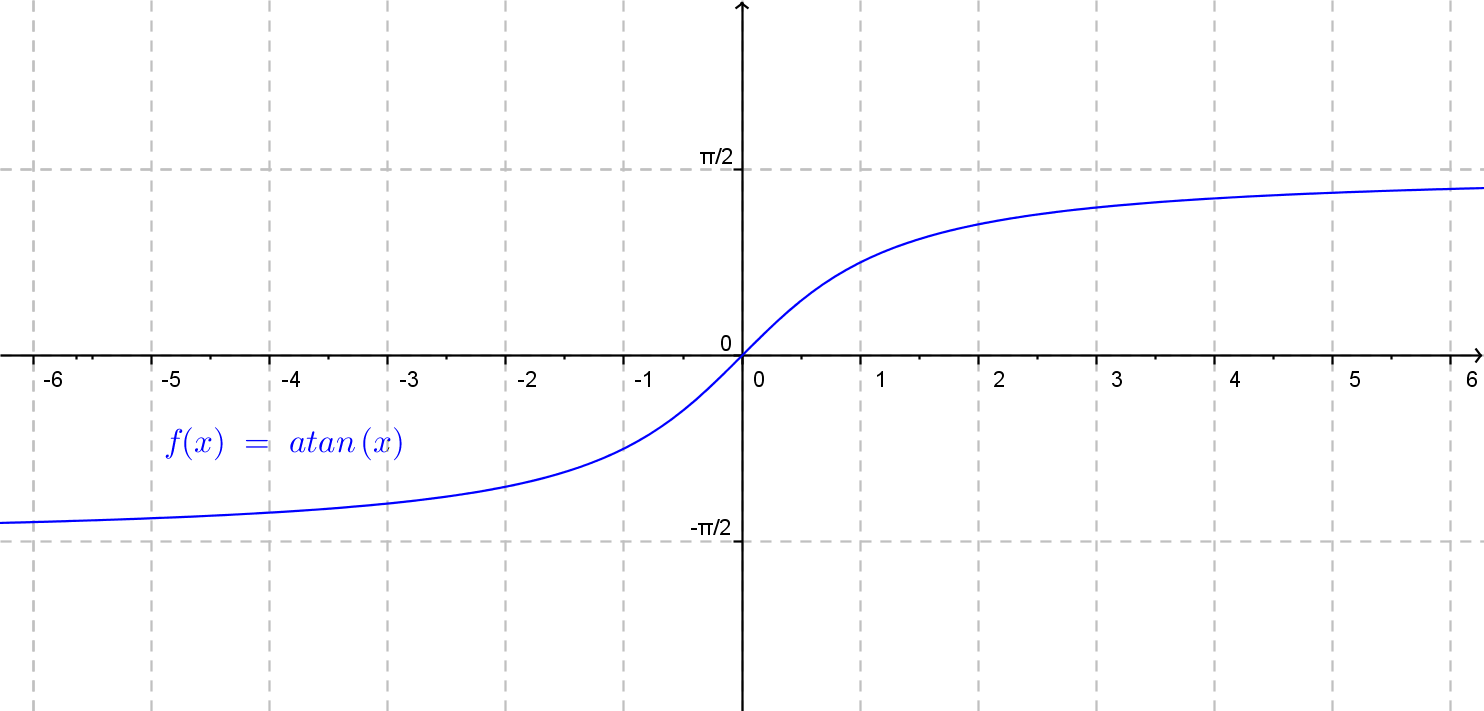
\includegraphics[height=8cm]{img/atangens.png}
  \caption{Graf funkce arkus tangens}
  \label{fig:atangens}
\end{figure}

Arkus tangens lze vyjádřit součtovým vzorcem 

\begin{center}
$ {\displaystyle \arctan x = \frac {\pi}{2} - \sum_{k=1}^{\infty} 
(-1)^k * \frac{1}{(2k-1)*x^{(2k-1)}}}$\end{center}

Tento vztah platí pro čísla, jejichž absolutní hodnota je větší než 1, a které
je nutné odečíst od periody. Pro čísla, jejichž absolutní hodnota je menší
než 1 lze použít vztah

\begin{center}
$ {\displaystyle \arctan x = \sum_{k=0}^{\infty} 
(-1)^k * \frac{x^{1+2k}}{1+2k}}$\end{center}

%=============================================================================
\subsection{Argument hyperbolického sinu}

Argument hyperbolického sinu (v projektu jako argsinh) je jednou z 
hyperbolomických funkcí. Jsou to funkce inverzní k funkcím hyperbolickým.
Definičním oborem i oborem hodnot funkce argsinh jsou všechna reálná čísla.

\begin{figure}[htbp]
  \centering
  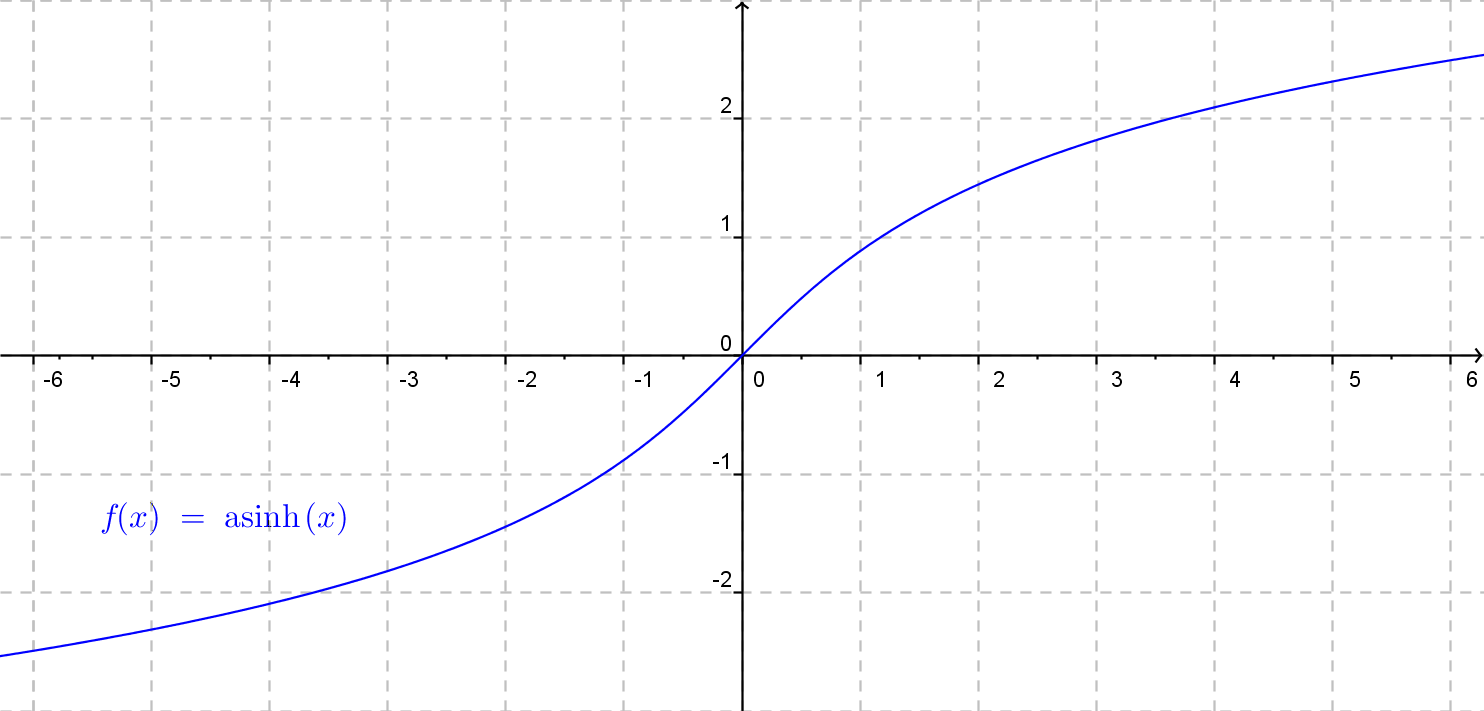
\includegraphics[height=8cm]{img/asinush.png}
  \caption{Graf funkce argument hyperbolického sinu}
  \label{fig:asinush}
\end{figure}

Pro výpočet funkce je potřeba přirozený logaritmus:

\begin{center}
$ {\displaystyle argsinh x = \ln(2x) + \sum_{k=1}^{\infty}
(-1)^{k-1}* \frac{(2k-1)!!}{2k*(2k!!)*x^{2k}}}$\end{center}


\section{Návrh řešení problému} \label{navrh}
%%%%%%%%%%%%%%%%%%%%%%%%%%%%%%%%%%%%%%%%%%%%%%%%%%%%%%%%%%%%%%%%%%%%%%%%%%%%%%

%=============================================================================
\subsection{Mocninná funkce}\label{rozsah}

Nekonečnou součtovou řadu mocninné funkce je potřeba přizpůsobit pro výpočet 
převedením na rekurentní vztah:

\begin{center}
$ {\displaystyle 1 + \frac{a*lnx}{1} + \frac{a*lnx^{2}}{2} + 
\frac{a*lnx^{3}}{3} + \ldots}$\end{center}

Pro získání nového členu z původního je potřeba vynásobit původním prvkem:

\begin{center}
$ {\displaystyle t_{y+1} = t_{y} * \frac{a*lnx}{i}}$\end{center}

Pro zjednodušení výpočtu rekurentním vztahem lze nahradit součin $a*lnx$ 
jako konstantu~\textit{r}. Součtová řada tedy bude:

\begin{center}
$ {\displaystyle 1 + \frac{r}{1} + \frac{r^{2}}{2} + 
\frac{r^{3}}{3}+ \ldots}$\end{center}


%=============================================================================
\subsubsection{Přirozený logaritmus}

Pro přirozený logaritmus platí součtový vzorec 
\begin{center}
$ {\displaystyle\ lnx = 2 \sum_{k=1}^{\infty} 
\frac{\frac{x-1}{x+1}^{2n-1}}{2n-1} 
= 2 * (\frac{x-1}{x+1} + \frac{1}{3}*\frac{x-1}{x+1}^{3} + 
\frac{1}{5}*\frac{x-1}{x+1}^{5} + \ldots ) }$\end{center}

\begin{figure}[htbp]
  \centering
  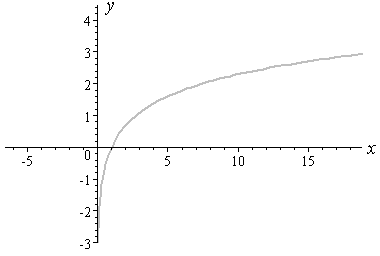
\includegraphics[height=6.cm]{img/ln.png}
  \caption{Graf funkce přirozený logaritmus}
  \label{fig:ln}
\end{figure}

Přirozený logaritmus je defionvaný pouze pro čísla v intervalu $(0;\infty)$,
při zadání záporné hodnoty tedy funkce počítající logaritmus vypíše hlášení o
tom, že pro dané číslo není tato funkce definována 
(\texttt{NaN} - \textit{Not a Number})\\

Součtové členy se u přirozeného logaritmu učují vzorcem 
\begin{center}
$ {\displaystyle t_{y+1} = t_{y} * 
(- \frac{(i-1)*(i-2)}{i^{2}*x^{2}})}$\end{center}

V intervalu $(0;1)$ je však $lnx$ záporný a při výpočtu těchto hodnot běžným
způsobem dochází k zacyklení programu. Při výpočtu těchto hodnot je tedy nutné
udělat úpravu výrazu $lnx$, aby při vypočtu těchto hodnot nedocházelo k 
chybám za pomocí vzoce $log_e x^{r} = r*ln_{e}x$ \\

Příklad: $\ln 0.5 = \ln (\frac{1}{0.5})^{-1} = -1 * \ln \frac{1}{0.5}$

%=============================================================================
\subsubsection{Odmocnina}

Jelikož s vysokými čísly mocninná funkce počítá nepřesně, je ve výpočtu 
logaritmu použito zjednodušení pomocí odmocniny, dosazením do téhož vzorcem,
jako při převodu převádějí čísel z intervalu $(0;1)$:

\begin{center}
$ {\displaystyle log_e x^{2} = 2*ln_{e}\sqrt{x^{2}}}$\end{center}

Odmocnina je vypočítaná pomocí Babylonské řady. Výpočet nového členu je daný 
vzorcem: 
\begin{center}
$ {\displaystyle t_{y+1} = \frac{1}{2} * (\frac{x}{t_y}+t_y)}$, přičemž
$t_0 = 1$\end{center}

%=============================================================================
\subsection{Arkus tangens}

Pro výpočet funkce arkus tangens jsou potřebné dvě součtové řady. Řady jsou
různé pro čísla, jejichž absolutní hodnota je menší než $1$, a čísla, jejichž
absolutní hodnota je větší než 1. Pro arkus tangens $1$ platí, že se rovná
$\frac{\pi}{4}$, pro $-1$ je arkus tangens roven $-\frac{\pi}{4}$ \\

Součtová řada pro $|x| > 1$:
\begin{center}
$ {\displaystyle \frac{\pi}{2} - \frac{1}{x} + \frac{1}{3x^{3}} - 
\frac{1}{5x^{5}} + \ldots}$\end{center}

Výpočet nového členu z předchozího se získá:

\begin{center}
$ {\displaystyle t_{y+1} = t_{y} * (-\frac{i-2}{x^{2}*i})}$\end{center}

Jelikož vynásobením prvního členu, tedy $\frac{\pi}{2}$ by nebyl získán
správný tvar druhého členu, je první člen již započítaný mimo součtový
rozvoj, a \textit{i} v iteracích se začíná počítat od $\textit{i} = 3$. 

Počet provedených operací je také možné zredukovat vytvořením proměnné 
(např. \texttt{x2}), ve
které bude uložena hodnota výrazu $x^{2}$. Není tedy potřeba zapisovat do 
výpočtu funkce
\texttt{x*x} \\

Jelikož s čísly v intervalu $(-1;1)$ součtová řada nepočítá přesně a dochází
k zacyklení programu, je potřeba tento interval počítat pomocí jiného rozvoje:

\begin{center}
$ {\displaystyle x - \frac{x^{3}}{3} + \frac{x^{5}}{5} - \frac{x^{7}}{7} + 
\ldots}$\end{center}

Získání nového členu z původního pak vypadá následovně:

\begin{center}
$ {\displaystyle t_{y+1} = t_{y} * (-\frac{(i-2)*x^{2}}{i})}$\end{center}

První člen součtového rozvoje bude započítán v celkové sumě ještě před cyklem.
Z toho důvodu bude v iteracích při počítání funkce v tomto intervalu 
\textit{i} opět začínat hodnotou $\textit{i} = 3$. I zde je také možno použít 
proměnnou \texttt{x2}, k uložení hodnoty \texttt{x*x} a snížit tak počet 
operací v cyklu

%=============================================================================
\subsection{Argument hyperbolického sinu}

Tato funkce potřebuje k výpočtu přirozený logaritmus. Pro výpočet logaritmu
byl použit stejný vzorec jako u mocninné funkce, s tím rozdílem, že se do
funkce odesílala hodnota $2*x$. Výsledek logaritmu je po vypočítání uložen do
celkové sumy, spolu s prvním členem součtového rozvoje, který je zde 
zapsán, jelikož při výpočtu rekurentním vztahem by se vynásobením prvního
členu nezískal správný následující člen. Proto je také \textit{i} číslováno na
začátku iterací od $4$

\begin{center}
$ {\displaystyle ln2x + \frac{1!!}{2*(2!!)*x^{2}} - \frac{3!!}{4*(4!!)*x^{4}}+
\frac{5!!}{6*(6!!)*x^{6}} + \ldots}$\end{center}

Výpočítání následujícího prvku z předchozího:

\begin{center}
$ {\displaystyle t_{y+1} = t_{y} * (- \frac{(i-1)(i-2)}{i^{2}*x^{2}})}$
\end{center}

%=============================================================================


%%%%%%%%%%%%%%%%%%%%%%%%%%%%%%%%%%%%%%%%%%%%%%%%%%%%%%%%%%%%%%%%%%%%%%%%%%%%%%
\section{Specifikace testů} \label{specif}
%%%%%%%%%%%%%%%%%%%%%%%%%%%%%%%%%%%%%%%%%%%%%%%%%%%%%%%%%%%%%%%%%%%%%%%%%%%%%%

%=============================================================================

Kromě ošetření extrémně malých a vysokých hodnot u výpočtu funkcí je třeba
v programu také ošetřit parametry, tedy zajistit, že se budou do funkcí
počítat pouze hodnoty, se kterými funkce dokáže počítat.

Například je nutné ověřit, zda na místě kde je možné zadat pouze jeden
parametr (konkrétně v části programu, který zajišťuje vypsání nápovědy) je
daný parametr zadaný správně, nebo jestli na místě kde je očekávaná číslice
není napsaný znak

\paragraph{Test 1:} Chybně zadané parametry $\longrightarrow$ Detekce chyby.

\vspace{1em}\begin{tabular}{ll} % ll = 2 sloupce zarovnane: left,left
vstup & očekávaný výstup \\
\hline
\verb|./proj2| & Byly nesprávně zapsané parametry. \\
\verb|./proj2 --help| & Byly nesprávně zapsané parametry. \\
\verb|./proj2 --argsinh| & Byly nesprávně zapsané parametry. \\
\verb|./proj2 --powxa -4| & Byly nesprávně zapsané parametry. \\
\end{tabular} 

\paragraph{Test 2:} Chybně zadaná přesnost $\longrightarrow$ Detekce chyby.
\begin{verbatim}
7x
-4
\end{verbatim} 

\paragraph{Test 3:} Chybně zadaný exponent mocninné funkce $\longrightarrow$ Detekce
chyby.
\begin{verbatim}
abc
-42
\end{verbatim} 

\paragraph{Test 4:} Neplatný znak na standartním vstupu $\longrightarrow$ Program vrátí hodnotu \texttt{NaN}
\begin{verbatim}
aleluja
)
5c5
\end{verbatim} 

\paragraph{Test 5:} Správnost výpočtu $\longrightarrow$ Předpokládaná správná
hodnota.

\vspace{1em}\begin{tabular}{ll} % ll = 2 sloupce zarovnane: left,left
 --powxa
vstup & očekávaný výstup \\
\hline
\verb|0^2| & 0.0000000000e+00 \\
\verb|-10^10| &  NaN\\
\verb|4^0.5| & 2.0000000000e+00 \\
\verb|200^100| & Inf \\
\verb|NaN^10| & NaN \\
\end{tabular}

\vspace{1em}\begin{tabular}{ll} % ll = 2 sloupce zarovnane: left,left
--arctg
vstup & očekávaný výstup \\
\hline
\verb|5| & 1.3734007669e+00 \\
\verb|0| & 0.0000000000e+00 \\
\verb|-52| & -1.5515679277e+00 \\
\verb|0.5| & -4.6364760900e-01 \\
\verb|NaN| & NaN \\

\end{tabular}

\vspace{1em}\begin{tabular}{ll} % ll = 2 sloupce zarovnane: left,left
--argsinh
vstup & očekávaný výstup \\
\hline         
\verb|5| & 2.3124383413e+00 \\
\verb|-5| & -2.3124383413e+00 \\
\verb|0| & 0.0000000000e+00 \\

\end{tabular}

%=============================================================================
\subsection{Ovládání programu}

Program funguje jako konzolová aplikace, má tedy pouze textové ovládání.
Program lze spouštět se čtyřmi typy parametrů

\vspace{1em}\begin{tabular}{ll} % ll = 2 sloupce zarovnane: left,left
parametr & funkce programu \\
\hline
\verb| -h | & vypsání nápovědy \\
\verb| --powxa | & mocninná funkce \\
\verb| --arctg | & arkus tangens \\
\verb| --argsinh | & argument hyperbolického sinu \\
\end{tabular}

%=============================================================================
\subsection{Volba datových typů}

V projektu je u funkcí použit datový typ \texttt{double}, stejně tak u většiny
proměnných, se kterými se v nich počítá. Také je zde použit datový typ
\texttt{boolean} u proměnných, které nábývají hodnot \texttt{TRUE}
nebo \texttt{FALSE}

%=============================================================================
\subsection{Vlastní implementace}

V hlavní funkci \texttt{main} se testují vstupní parametry, a ověřuje se jejich
správnost. Pakliže jsou parametry zadány v souladu s požadavky programu,
očekává program vstupní hodnotu, se kterou program výpočítá funkci, která byla
zvolena v parametrech programu, jestliže parametry nejsou správně zadané,
uživatel je na jejich nesprávnost upozorněn chybovým hlášením. Po vypočítání
funkce program opět očekává vstupní hodnotu pro další výpočet. Tento cyklus
probíhá, dokud není zadáno \texttt{EOF}

%%%%%%%%%%%%%%%%%%%%%%%%%%%%%%%%%%%%%%%%%%%%%%%%%%%%%%%%%%%%%%%%%%%%%%%%%%%%%%
\section{Závěr} \label{zaver}
%%%%%%%%%%%%%%%%%%%%%%%%%%%%%%%%%%%%%%%%%%%%%%%%%%%%%%%%%%%%%%%%%%%%%%%%%%%%%%

Program slouží k výpočtu tří matematických funkcí - mocninné funkce s realným
exponenetem, funkce arkus tangens a argumentu hyperbolického sinu.
V parametrech funkce uživatel stanoví, s jakou přesností chce počítat
vybranou funkci.

Pro správné vypracování programu bylo nutné pochopit v analytické části
princip jednotlivých operací a celkový princip výpočtu. Důležité taktéž bylo
správně zvolit řadu pro výpočet funkcí a zjistit, v jakýchh intervalech funkce
nejrychleji konvergují

%%%%%%%%%%%%%%%%%%%%%%%%%%%%%%%%%%%%%%%%%%%%%%%%%%%%%%%%%%%%%%%%%%%%%%%%%%%%%%
% seznam citované literatury: každá položka je definována příkazem
% \bibitem{xyz}, kde xyz je identifikátor citace (v textu použij: \cite{xyz})
\begin{thebibliography}{1}

% jedna citace:
\bibitem{kalendar}
BARTSCH, H.-J.; HOLFORD-STREVENS, L.: \emph{Matematické vzorce. } Praha:
Mladá fronta, třetí vydání, 1996, 831 s., 
ISBN 80-204-0607-7.


\end{thebibliography}
%%%%%%%%%%%%%%%%%%%%%%%%%%%%%%%%%%%%%%%%%%%%%%%%%%%%%%%%%%%%%%%%%%%%%%%%%%%%%%
% přílohy
\appendix

\section{Metriky kódu} \label{metriky}
\paragraph{Počet souborů:} 1 soubor
\paragraph{Počet řádků zdrojového textu:} 494 řádků
\paragraph{Velikost statických dat:} 300B
\paragraph{Velikost spustitelného souboru:} 9330B (systém Linux, 32 bitová
architektura, při pře\-kladu bez ladicích informací)


\end{document}
